\chapter{Introduction}\label{cha:intro}

The goal of this report is to describe the process of design and implementation of the Final Undergraduate Project \textit{"SORELCOM: Design and Development of a semantic geospatial web and mobile application"}.

This project has been carried by Aimar Rodr\'iguez Soto, 4th year student of an undergraduate degree in computer science engineering.

The different chapters that form this document are the following:

\begin{enumerate}
	\item \textbf{Introduction:} Brief descriptions of the contents of the report, as well as a small introduction to the concepts of Semantic Web and GIS System.
	
	\item \textbf{Project goals:} The goals, the limits, the tasks to perform, working methodologies and the working plan are presented.
	
	\item \textbf{Technological research:} Detailed description of the different technologies used throughout the project, thus presenting the results of the technological research.
	
	\item \textbf{Requirement Specification:} Requirements of the project and the final product are listed and analyzed.
	
	\item \textbf{Design specification:} Design considerations of the project are described, both from the technological and the user experience point of views.
	
	\item \textbf{Development:} Usage of the described technologies, solutions to the common problems and details about the implementation are given.
	
	\item \textbf{Testing:} Testing plan, tools, methodologies and special test cases are described. 
	
	\item \textbf{User guide:} Document explaining how to use the developed tools and platforms at a user level.
	
	\item \textbf{Conclusions and future lines of work:} Analysis of the results of the project and further considerations, such as improvements and future work to be done.
\end{enumerate}

\section{The Semantic Web}

The semantic web is a extension of the current web in which information is given well-defined meaning, better enabling computers and people to work in cooperation. \cite{berners2001semantic}

The idea behind the semantic web is to bring meaning and structure to the contents of web pages, creating an environment where software agents can roam the web carrying out sophisticated tasks for end users. Thanks to the semantic web, this agents will be able to understand the relationships among the information on a web page, beyond simply identifying certain keywords. 

This machine-readable web of data is based standard languages which allow a uniform representation of the information throughout the different semantic data sources. Through this common infrastructure it is possible to share and process information in a relatively simple way, enabling better solution to the usual problem of searching through the web of information. In short, the Semantic Web attempts to give meaning and structure to the contents on the web, allowing computers to better understand this information to do more useful work.

\subsection*{The fundamentals}

The Semantic Web is based on standard formats used for a universal representation and manipulation of data. This standards are the following:

\begin{description}
	\item[RDF:] The Resource Description Framework (RDF) is a standard language for representing information about resources in the World Wide Web. Resources can be anything, including documents, people, physical object and abstract concepts. \cite{rdfprimer10}
	
	\item[OWL:] The Web Ontology Language (OWL) is a semantic markup language for creating and sharing ontologies \cite{bechhofer2009owl}.  It is used to define ontologies when the content needs to be processed by applications or agents, instead of just presented to people \cite{mcguinness2004owl}. 

	\item{SPARQL:} the SPARQL Protocol and RDF Query Language is a language designed to make queries over resources in RDF format \cite{sparqlquery}. 
\end{description}

The idea of the semantic web is based on a stack architecture, illustrated on figure \ref{fig:semwebstack}. This stack includes more layers than the mentiones, such as RDF Schema (RDFS) and the eXtensible Markup Language (XML). For further detail into these technologies and their role in the semantic web refer to chapter \ref{cha:research}.

\begin{figure}
  \centering
  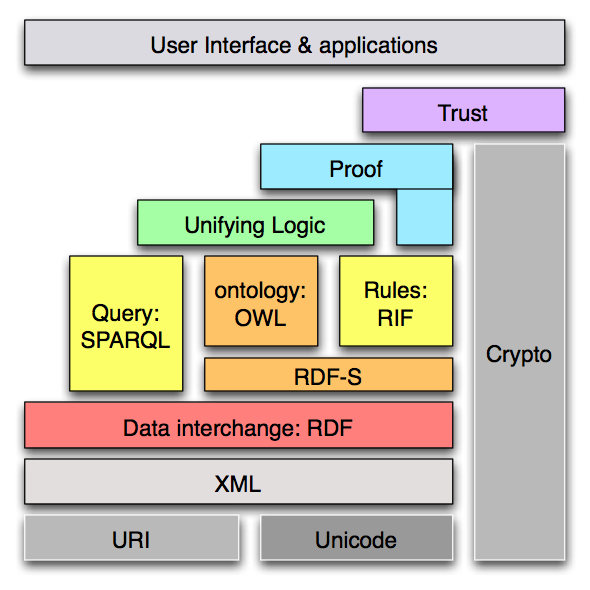
\includegraphics[width=.5\textwidth]{fig/semwebstack}
  \caption{The semantic web architecture}
  \captionsetup{font={footnotesize,bf,it}}
  \caption*{source: \url{http://www.w3.org/2006/Talks/1023-sb-W3CTechSemWeb/\#(19)}}
  \label{fig:semwebstack}
\end{figure} 

\subsection{Introduction to RDF}

RDF provides a framework for representing information which can be exchanged between application without loss of meaning and it is intended for situation in which this information needs to be processed by machines instead of displayed to humans, thus making it fitting for the goals of The Semantic Web  \cite{rdfprimer11}.

This framework has several uses, such as:

\begin{itemize}
	\item Adding machine readable information to web pages, enabling them to be displayed in enhanced formats or to be processed by other agents.
	\item Enriching a database by linking it to third party datasets.
	\item Interlinking API feeds, so that clients can easily discover how to access more information.
	\item Using datasets labeled as Linked Data to build aggregations of data around specific topics or concepts.
\end{itemize} 

RDF information is stored in triples which follow a simple subject-predicate-object pattern. One example of RDF triples which represent knowledge about a person named Bob can be found in listing \ref{lst:bobtriples}. Note that in this set of triples, most attributes appear between brackets, these are International Resource Identifiers (IRIs) linking to other resources, while the other attributes are just literal values. 

\begin{listing}\centering
  \begin{minipage}{.4\textwidth}
    \begin{minted}[linenos=true,mathescape,gobble=6]{xml}
     <Bob> <is_named> "Bob"
     <Bob> <is_a> <Person>
     <Bob> <is_a> <Student>
     <Bob> <knows> <Alice>
     <Bob> <is_interested_in> <Computer_Science>
    \end{minted}
  \end{minipage}
  \caption{Set of triples in pseudocode representing Bob.}\label{lst:bobtriples}
\end{listing}

These IRIs are identifiers for resources on the Semantic Web. Up to now the concepts of URI and IRI have been mixed, to make it clear, an IRI is a generalization of an URI. The form of a IRI is similar to that of the Uniform Resource Locators (URL) used in the World Wide Web, in fact these last are just a form of IRI, thus they look like the following:  \url{http://dbpedia.org/resource/Leonardo_da_Vinci}
 

\subsection{Introduction to Ontologies}

In the Semantic Web, vocabularies or ontologies define the concepts and relationships used to describe and represent a certain area of knowledge, they define the terms that can be used on a application, the possible relationships and their constraints. They are used to help data integration when ambiguity may exist between terms in different datasets, or simply to organize knowledge \cite{w3contologies}.

According to Tom Grubber \cite{gruber1993ontology} An ontology is a formal specification of a shared conceptualization. The concept of Ontology comes from the field of philosophy, however they have been adopted into Artificial Intelligence and Knowledge Representation \cite{chandrasekaran1999ontologies}. Since ontologies are used to create conceptual structure on a domain, they can be used by software for problem solving and reasoning among other tasks.

We can find three types of ontologies:

\begin{description}
	\item[Top-level ontologies]: Describe very general notions which are independant of a particular domain and are applicable to different areas, for example; time, space, events, etc.
	
	\item[Domain ontologies]: The knowledge represented in these ontologies is particular to a certain field of knowledge, such as computers, persons, forestry, etc.	They provide information about concepts in the domain and about the theories governing the domain.
	
	\item[Application ontologies]: This is the least general type of ontology. It describes knowledge specific to a certain a application or task, due to this, they are useful for problem solving.
\end{description}

\section{Introduction to GIS systems}

A Geographical Information System (GIS) integrates hardware, software and data for capturing, managing and displaying all forms of geographically referenced information \cite{esrigis} A GIS provides a framework for gathering and organizing spatial data and related information so it can be displayed and analyzed.

Data on such a system is a digital representation of real world objects. Since this kind of data can be divided into two abstractions, discrete objects (a house, a park) or continuous fields (elevation), two methods are used to store data of this abstractions: Raster and Vector. \cite{giswikigis}

\subsection*{Raster}

Raster data types consist of rows and columns of cells each of them storing a single value, in the say way that a image is composed by pixels. In fact, a Raster data type is, in essence, a type of digital image represented in grids. On a Raster Image each pixels stores a color value which represents certain data, for example, the amount of rain in that region.

This kind of data may be stored in different ways, for example, as a regular .JPEG image or directly in a relational database.

\subsection*{Vector}

Vector data is used to express geographical features, which are represented as geometrical shapes of different types.

\begin{itemize}
	\item \emph{Points:} They are used to describe features that can be represented with a single point, that is, the simplest of features, for example, the location of a monument, the peak of a mountain, etc.
	\item \emph{Lines or polylines:} They are used to represent linear features, such as rivers, roads, trails, etc. It is possible to measure distance on line features.
	\item \emph{Polygons:} They are used for the representation of features that cover a particular area of the earth's surface, for example, a country. It is possible to measure area and perimeter of polygons.
\end{itemize}










